\chapter{Dashboard BI, Trực quan hóa và Đề xuất Quyết định}
\label{ch:bi_quyetdinh}

\section{Kiến trúc Ứng dụng BI 5 Trang và Lập luận Giá trị}
Hệ thống cung cấp đồng thời 2 lớp khai thác BI: \textbf{Amazon QuickSight (4 Sheets)} đọc trực tiếp qua Neon BI Mirror và ứng dụng web \textbf{Streamlit Multipage 5 trang tiếng Việt} (\texttt{src/streamlit/app.py}), sử dụng \textbf{SQL aggregation pushdown} trên PostgreSQL (\texttt{0.08--0.48s}/query), hỗ trợ \textbf{7 bảng màu giao diện}, bảo toàn đa ĐVT (\texttt{IRPD}), cấm cộng trùng \texttt{order\_count} ở grain sản phẩm--ngày và xuất CSV giữ nguyên dấu UTF-8:
\begin{enumerate}[leftmargin=1.5em]
  \item \textbf{Trang 1 -- Cửa Hàng \& Mặt Hàng:} 6 thẻ KPI phân tách kỳ so sánh, tăng trưởng MoM, đóng góp biến động số học và bảng tách ĐVT.
  \item \textbf{Trang 2 -- Cụm CH \& Bản Đồ:} Phân tích Same-Store, ma trận Doanh thu $\times$ Biên lợi nhuận gia quyền, danh sách cửa hàng cần xem xét (\textit{Watchlist}) và bản đồ cụm cửa hàng Châu Âu.
  \item \textbf{Trang 3 -- Thời Tiết \& Mùa Vụ:} Bộ lọc cục bộ ô Nhiệt độ $\times$ Mức mưa chuẩn hóa theo \texttt{active\_store\_days}, cảnh báo ô cỡ mẫu nhỏ (\texttt{n < 30}).
  \item \textbf{Trang 4 -- So Sánh Kỳ \& Danh Mục:} Dịch chuyển cơ cấu (\textit{Mix Shift}), Treemap, Top 15 nhà sản xuất \texttt{IRPD} và chuỗi lịch sử 8 nhóm ATC.
  \item \textbf{Trang 5 -- Dự Báo Nhu Cầu (ML):} Tab nghiệp vụ hiển thị Fan Chart \texttt{52W/365D} kèm dải tin cậy 80\% Split CQR, biểu đồ thanh ngang \texttt{TreeSHAP} dịch sang tiếng Việt; và Tab kiểm chứng đối chuẩn Paper 2024, Ablation ERA5, 4-Fold Stability và \texttt{DM'}.
\end{enumerate}

\begin{figure}[H]
\centering
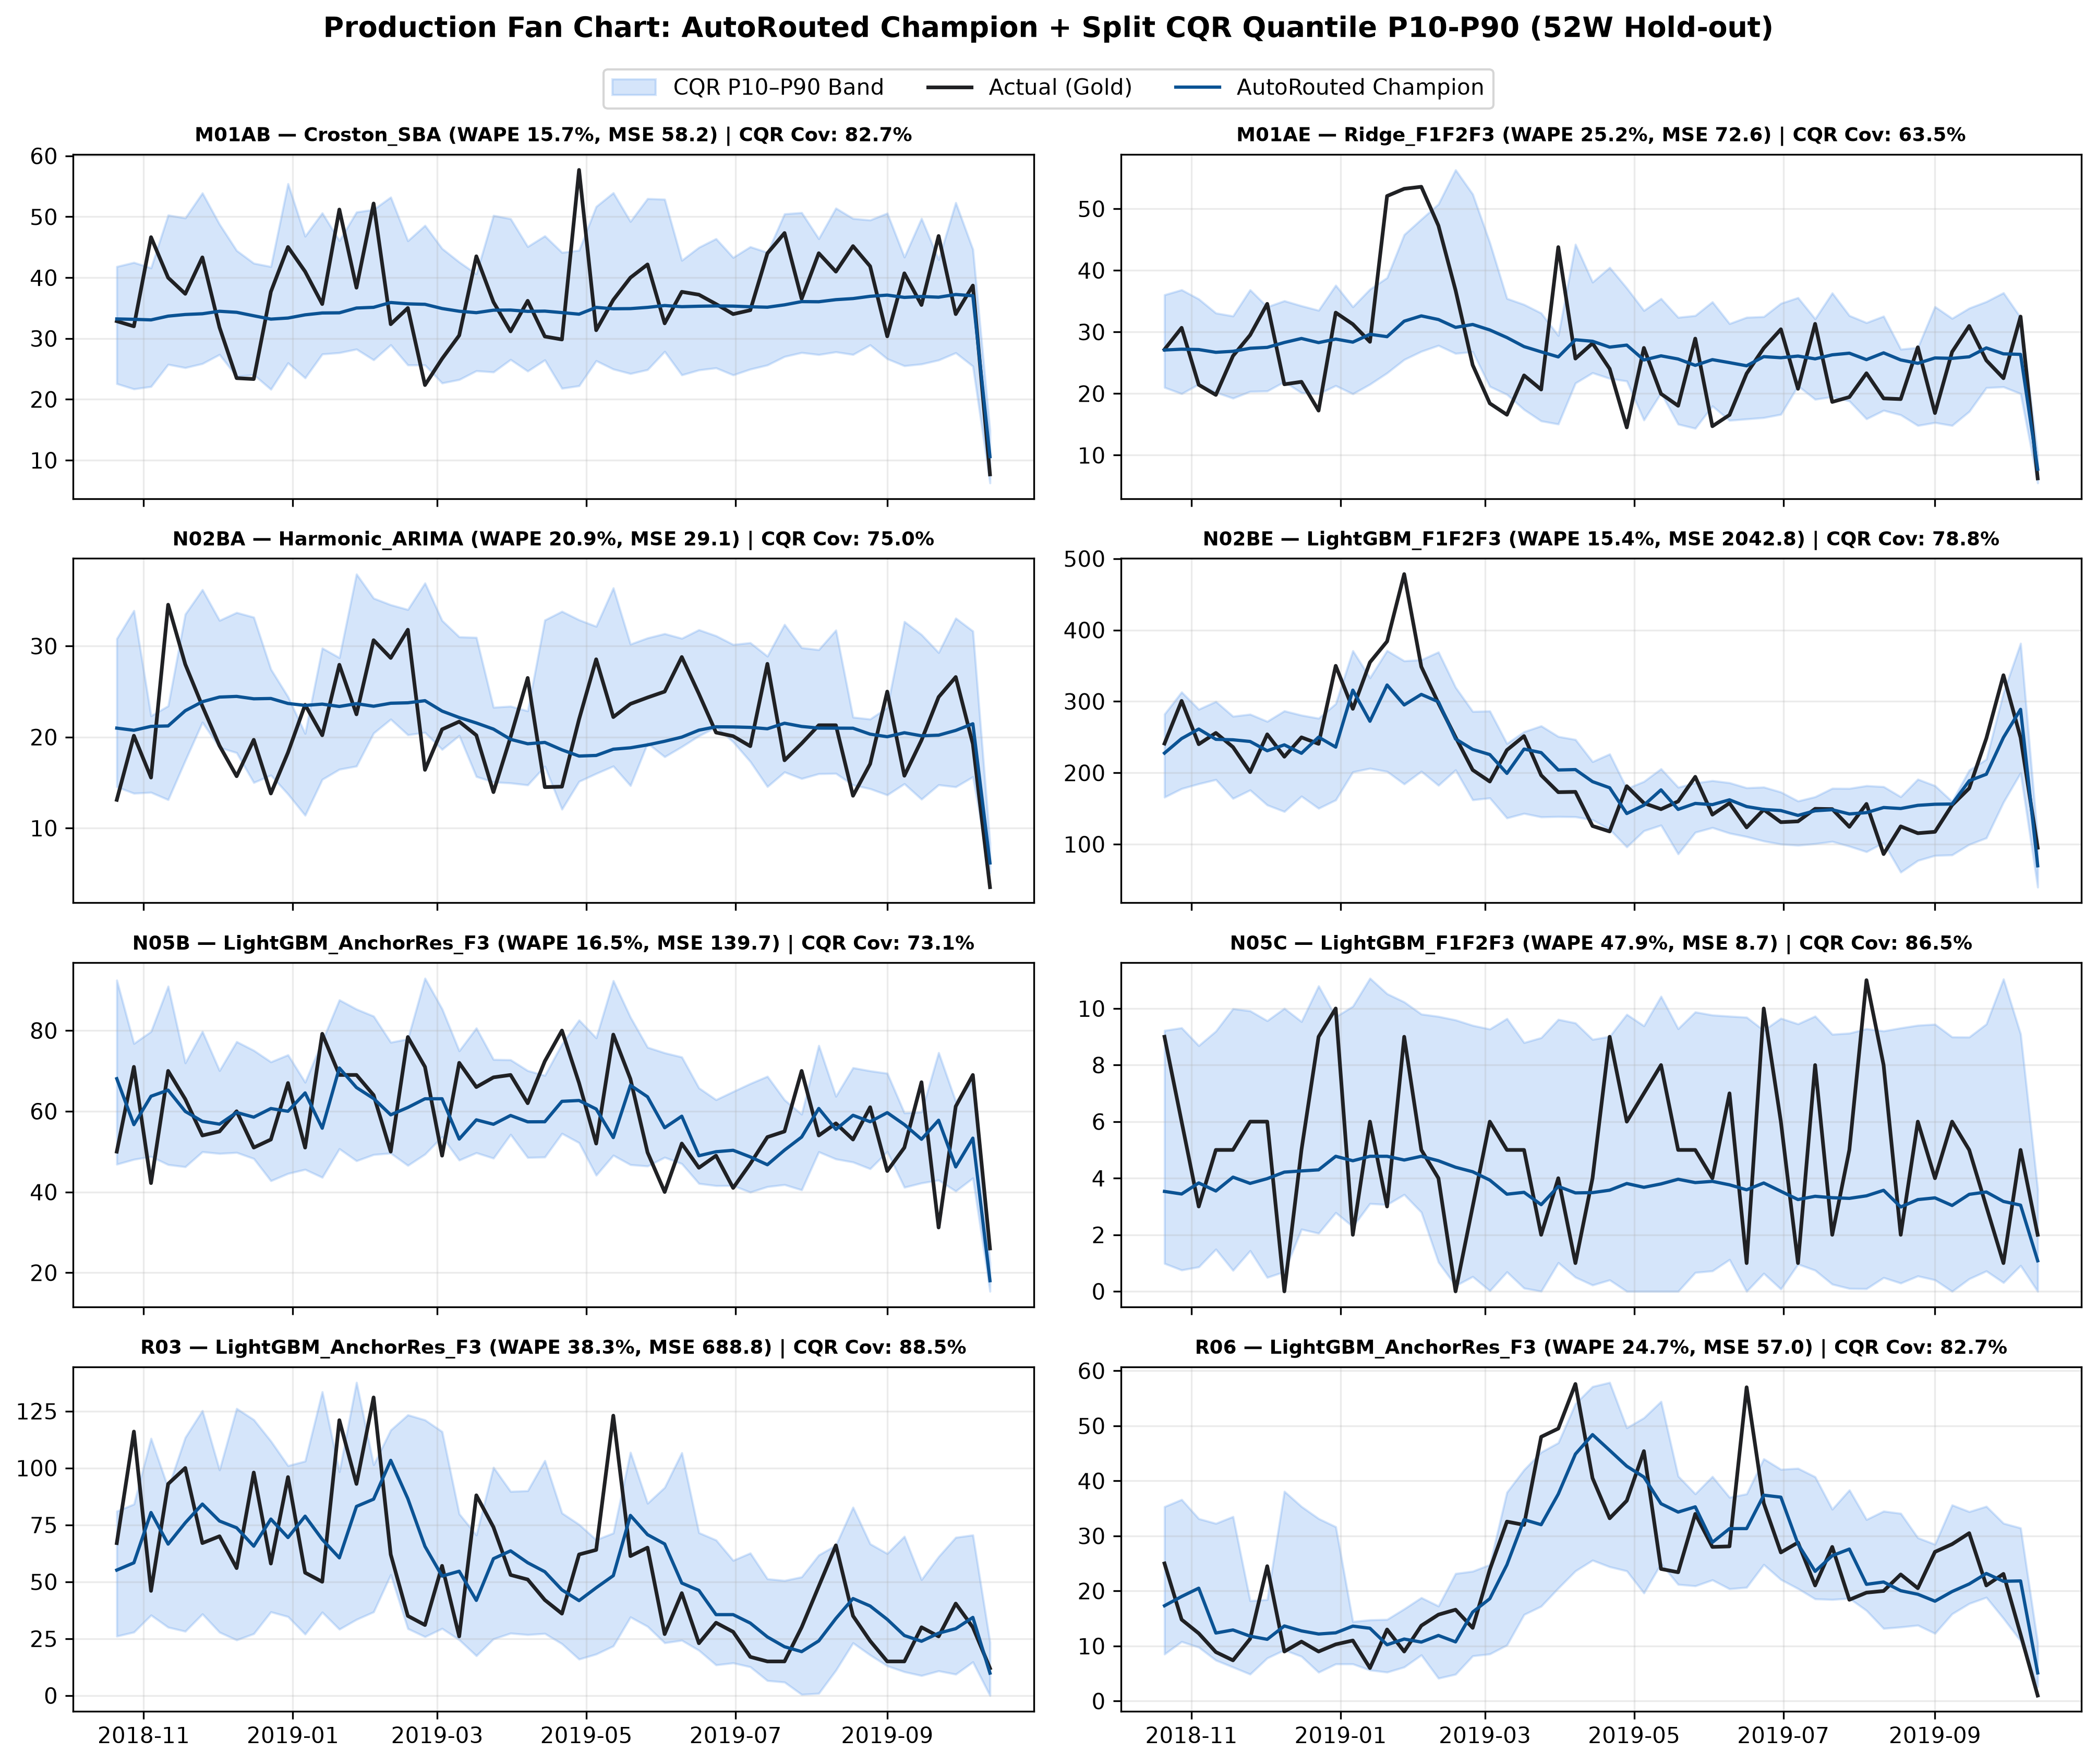
\includegraphics[width=\textwidth]{../../artifacts/forecasting/eval_fanchart_52w.png}
\caption{Minh họa Fan Chart dự báo 52 tuần cuối kèm dải tin cậy Split CQR ($P_{10}$--$P_{90}$) tích hợp trên Trang 5 Streamlit}
\label{fig:eval_fanchart}
\end{figure}

\begin{table}[H]
\centering
\caption{Khung chèn ảnh chụp màn hình 5 trang ứng dụng Streamlit BI thực tế (Nhóm tự chụp trước khi nộp)}
\label{tab:ui_screenshots}
\renewcommand{\arraystretch}{1.35}
\begin{tabularx}{\textwidth}{|c|p{0.28\textwidth}|X|}
\hline
\textbf{Trang} & \textbf{Tên giao diện} & \textbf{Minh chứng ảnh chụp màn hình} \\
\hline
Trang 1 & Cửa Hàng \& Mặt Hàng & [Chờ nhóm chụp \& chèn \texttt{screenshot\_page1.png}] \\
\hline
Trang 2 & Cụm CH \& Bản Đồ & [Chờ nhóm chụp \& chèn \texttt{screenshot\_page2.png}] \\
\hline
Trang 3 & Thời Tiết \& Mùa Vụ & [Chờ nhóm chụp \& chèn \texttt{screenshot\_page3.png}] \\
\hline
Trang 4 & So Sánh Kỳ \& Danh Mục & [Chờ nhóm chụp \& chèn \texttt{screenshot\_page4.png}] \\
\hline
Trang 5 & Dự Báo Nhu Cầu (ML) & [Chờ nhóm chụp \& chèn \texttt{screenshot\_page5.png} (Tab 1 + Tab 2)] \\
\hline
\end{tabularx}
\end{table}

\section{Nhận xét Định lượng Rút ra từ Số liệu}
Dựa trực tiếp trên số liệu kiểm chứng của hệ thống, nhóm rút ra \textbf{4 nhận xét trọng tâm}:
\begin{enumerate}[leftmargin=1.5em]
  \item \textbf{Phân hóa chiến lược mô hình theo đặc tính ATC:} Không có mô hình đơn lẻ nào tối ưu cho mọi nhóm thuốc; \texttt{Ridge} nổi trội với chuỗi trôi mượt (\texttt{M01AB MSE 52.68}, \texttt{N05B MSE 118.65}), \texttt{LightGBM AnchorRes} phá ngưỡng trần cây cho nhóm chủ lực (\texttt{N02BE MSE 1392.20} vs Paper XGB \texttt{1518.56}), còn \texttt{Croston-SBA} phù hợp với nhóm bán thưa \texttt{N05C} (\texttt{MSE 7.76}).
  \item \textbf{Giá trị thực chứng của dữ liệu Thời tiết ERA5 (\texttt{F3}):} Cụm 7 biến ERA5 giúp giảm sai số trên \texttt{5/8} nhóm tuần (đạt ý nghĩa \texttt{DM' p = 0.0339} tại \texttt{N05B} và \texttt{p = 0.0096} tại \texttt{N05C Daily}) và đóng góp \texttt{11.3\%--25.9\%} tổng \texttt{|TreeSHAP|} (nổi bật: \texttt{daylight\_duration\_s = 8.06} tại \texttt{N02BE}; \texttt{temp\_mean\_lag1 = 2.35} tại \texttt{R03}; \texttt{daylight + humidity\_lag1} chiếm \texttt{25.9\%} tại \texttt{R06}).
  \item \textbf{Cải thiện độ tin cậy cảnh báo bất định:} Nhờ hiệu chuẩn Split CQR trên tập Validation, độ phủ thực nghiệm 80\% tăng từ \texttt{71.7\%} lên \texttt{78.8\%} (đặc biệt \texttt{N02BE} từ \texttt{55.8\%} lên \texttt{78.8\%}).
  \item \textbf{Toàn vẹn thước đo BI đa nguồn:} Khóa cộng gộp sản lượng đa ĐVT tại \texttt{IRPD}, tách rời giá trị \texttt{0} với \texttt{Không có dữ liệu} và dùng \texttt{WAPE/MASE} thay thế \texttt{MAPE} giúp loại bỏ sai số bóp méo quyết định quản trị.
\end{enumerate}

\section{Đề xuất Quyết định, Chi phí, Rủi ro và Điều kiện Áp dụng}
\begin{table}[H]
\centering
\caption{Đề xuất hành động vận hành gắn với Chi phí, Rủi ro và Điều kiện áp dụng}
\label{tab:decisions}
\renewcommand{\arraystretch}{1.22}
\begin{tabularx}{\textwidth}{|p{0.23\textwidth}|p{0.25\textwidth}|p{0.25\textwidth}|X|}
\hline
\textbf{Hành động đề xuất} & \textbf{Cơ sở số liệu BI/ML} & \textbf{Rủi ro \& Hạn chế} & \textbf{Điều kiện áp dụng \& Chi phí} \\
\hline
Ưu tiên dự trữ chủ động nhóm mùa đông (\texttt{N02BE}) \& dị ứng (\texttt{R06}) theo dải $P_{90}$ trước biến động nắng/ẩm & \texttt{N02BE} (\texttt{ACF52=0.53}, WAPE \texttt{12.96--15.44\%}), \texttt{R06} (\texttt{25.9\% SHAP} thời tiết), độ phủ CQR \texttt{78.8--82.7\%} & Rủi ro dư tồn kho nhẹ nếu dự báo theo $P_{90}$ kéo dài trong điều kiện thời tiết đổi chiều đột ngột & Con người duyệt cuối (\textit{Human-in-the-loop}); gần như \texttt{\$0} chi phí API ERA5/Serverless thêm. \\
\hline
Không tự động hóa đặt hàng trên nhóm bán thưa \texttt{N05C} \& hô hấp \texttt{R03} & \texttt{N05C} có \texttt{67.9\%} ngày \texttt{= 0} (WAPE \texttt{44--48\%}); \texttt{R03} biến động \texttt{CV$^2$=0.82} & Sai số tương đối cao và tập dữ liệu Gold hiện \textbf{chưa có tồn kho thực} & Chỉ dùng kết hợp biên CQR ($P_{10}$--$P_{90}$) làm tín hiệu tham khảo cho dược sĩ phụ trách. \\
\hline
Tách riêng báo cáo theo ĐVT (\texttt{IRPD}) và rà soát \textit{Watchlist} biên LN thấp (\texttt{ONYX}) & \texttt{IRPD} có nhiều ĐVT chưa có hệ số \texttt{base\_qty}; \texttt{ONYX} theo dõi được biên LN gia quyền EUR & Khuyến mãi chỉ quan sát mô tả trên \texttt{SYNTHETIC}, không khẳng định nhân quả & Chỉ cần giữ quyền đọc \path{bi_reader} trên Neon \path{quick_gold_md01}. \\
\hline
\end{tabularx}
\end{table}
